% !TEX root = ../report.tex
\section{Brokered Authentication}

\begin{figure}[H]
\centering
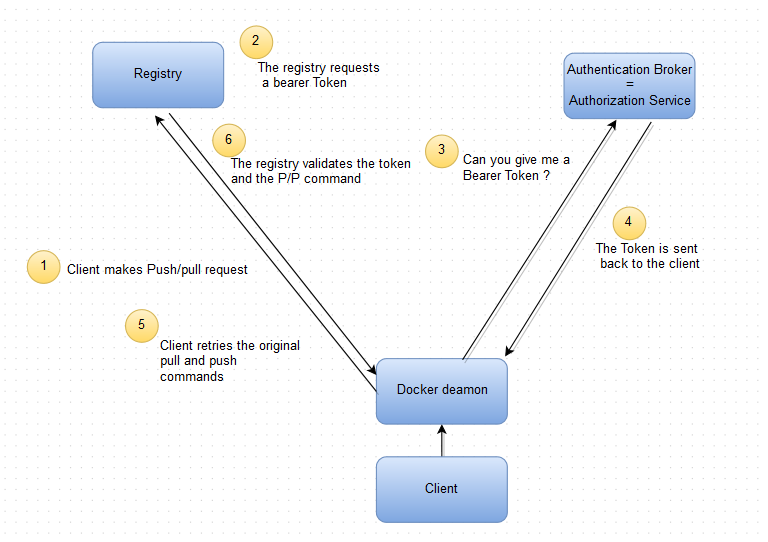
\includegraphics[scale=0.7]{5-patterns/images/Authentication.png}
\caption{Authentication process of the Docker registry }
\label{fig:auth-process}
\end{figure}
\begin{patdescription}

\item[Traceability]
From the v2 of Docker the authentication is done through a central service. \\
The Brokered Authentication pattern can be deducted from the source code through the "auth.go" and the "token.go" files from the Docker Registry Github Repository. \\
Docker Authentication \cite{dockauth}
%https://docs.docker.com/registry/spec/auth/jwt/

The main functions for authentication are : \\
\begin{mynesteditemlist}
\item func tryV2TokenAuthLogin(authConfig *types.AuthConfig, params map[string]string, registryEndpoint *Endpoint)
\item func loginV2(authConfig *types.AuthConfig, registryEndpoint *Endpoint, scope string) 
\end{mynesteditemlist}
% They allow the 

%TODO joris: remove quote
\begin{quote}
This service is used by the official Docker Registry to authenticate clients and verify their authorization to Docker image repositories.
\end{quote}

\item[Source]
Brokered Authentication Pattern\cite{brokeredauth} \\
%https://msdn.microsoft.com/en-us/library/ff650014.aspx

\item[Issue] The Docker Registry needs an authentication system in order to ensure security of pulling and pushing images.

\item[Assumptions/Constraints] 

  %  \quote {Registry clients which can understand and respond to token auth challenges returned by the resource server. \\
   % An authorization server capable of managing access controls to their resources hosted by any given service (such as repositories in a Docker Registry). \\
   % A Docker Registry capable of trusting the authorization server to sign tokens which clients can use for authorization and the ability to verify these tokens for single use or for use during a sufficiently short period of time.} \\

%"An authentication broker with a centralized identity store assumes the responsibility for authenticating the consumer and issuing a token that the consumer can use to access the service."
\item[Solution] 
An authentication broker that both parties trust independently, issues a security token to the client. The client can use this token to authenticate himself. This means that there is no direct relationship between the user and the registry.

By using the Brokered Authentication the access to the Docker Registry is controlled for each user.

%The consumer submits a request with credentials to the authentication broker (1), which the broker authenticates against a central identity store (2). The broker then responds with a token (3) that the consumer can use to access Services A, B, and C (4), none of which require their own identity store.  % sum up in my own words
% Explaining the steps
%In the Docker registry case the central identity store is the Authorization service from the picture.

\item[Rationale] 

\item[Implication] After the integration of the Brokered authentication the textbf{Security} for the registry is ensured. % why BLABLABLA but single point of failure
The authentication broker manages trust centrally. This eliminates the need for each client and service to independently manage their own trust relationships.

\item [Related Patterns]
Shared/Active Repository Pattern

\end{patdescription}

